%--------------------------------------------------------------------------
% Document geometry % Page margins
%--------------------------------------------------------------------------
\usepackage[margin=1in,headsep=10pt,a4paper]{geometry}

%--------------------------------------------------------------------------
% MinionPro fonts
%--------------------------------------------------------------------------
\IfFileExists{MinionPro.sty}{%
  \usepackage{MnSymbol}
  \usepackage{MinionPro}
  \usepackage{MyriadPro}
}{%
  \usepackage[T1]{fontenc}
  \usepackage{newtxtext}
  %\usepackage{eulervm}
  \usepackage{amssymb}%needed for \mathbb
}

%--------------------------------------------------------------------------
% Color scheme used in this book
%--------------------------------------------------------------------------
\usepackage{xcolor} % Required for specifying colors by name
\definecolor{ocre}{RGB}{243,102,25} % Define the orange color used for highlighting throughout the book
\definecolor{dkgreen}{rgb}{0,0.6,0}
\definecolor{delim}{RGB}{20,105,176}
\definecolor{background}{HTML}{EEEEEE}
\definecolor{Red}{rgb}{0.8666,0.03137,0.02352}
\definecolor{Blue}{rgb}{0.00784,0.67059,0.91764}
\definecolor{Darkgreen}{rgb}{0,0.68235,0}
\definecolor{Green}{rgb}{0,0.8,0}
\definecolor{Royalblue}{rgb}{0,0.2,0.91764}
\definecolor{Brickred}{rgb}{0.644541,0.164065,0.164065}
\definecolor{Brown}{rgb}{0.6,0.4,0.4}
\definecolor{Orange}{rgb}{1,0.647059,0}
\definecolor{Indigo}{rgb}{0.746105,0,0.996109}
\definecolor{Violet}{rgb}{0.308598,0.183597,0.308598}
\definecolor{Lightgrey}{rgb}{0.762951,0.762951,0.762951}
\definecolor{Darkgrey}{rgb}{0.503548,0.503548,0.503548}
\definecolor{Pink}{rgb}{1,0.6,0.6}
\definecolor{DarkBlue}{rgb}{0,0.08,0.45}
\definecolor{OliveDrab}{rgb}{0.41961,0.55686,0.13725}
\definecolor{LightMagenta}{cmyk}{0.1,0.8,0,0.1}
\definecolor{OliveD}{HTML}{6B8E23}
\definecolor{authorNoteColor}{rgb}{.8,0,0}
\newcommand{\Ochre}{\color{ocre}}
\newcommand{\Red}{\color{Brickred}}
\newcommand{\Blue}{\color{Royalblue}}
\newcommand{\Green}{\color{Darkgreen}}
\newcommand{\DarkGreen}{\color{Darkgreen}}
\newcommand{\Violet}{\color{Violet}}
\newcommand{\Indigo}{\color{Indigo}}
\newcommand{\Orange}{\color{Orange}}
\newcommand{\Brown}{\color{Brown}}
\newcommand{\OliveD}{\color{OliveD}}
\newcommand{\Pink}{\color{Pink}}


%--------------------------------------------------------------------------
% Bibliography : biblatex does not work with tufte-book
%--------------------------------------------------------------------------
\usepackage[style=numeric,
            citestyle=numeric-comp,
            sorting=none,
            sortcites=true,
            autopunct=true,
            babel=hyphen,
            hyperref=true,
            abbreviate=false,
            backref=true,
            backend=biber]{biblatex}
\addbibresource{../Bibliography.bib} % BibTeX bibliography file
\defbibheading{bibempty}{}

%--------------------------------------------------------------------------
% Graphics
%--------------------------------------------------------------------------
\usepackage[pdftex]{graphicx}
\DeclareGraphicsExtensions{{.png},{.pdf},{.jpg},{jpeg}}
\graphicspath{ {../figures/}}
\setkeys{Gin}{width=\linewidth,totalheight=\textheight,keepaspectratio}

%--------------------------------------------------------------------------
% Links
%--------------------------------------------------------------------------
\usepackage{hyperref}
\hypersetup{pdftex, colorlinks=true, linkcolor=blue, citecolor=blue, filecolor=blue, urlcolor=blue, pdftitle=, pdfauthor= , pdfsubject=, pdfkeywords=}

%--------------------------------------------------------------------------
% Code listing
%--------------------------------------------------------------------------
\usepackage{listings}

\lstset{ %
  basicstyle=\scriptsize\ttfamily,           % the size of the fonts that are used for the code
  backgroundcolor=\color{white},      % choose the background color. You must add \usepackage{color}
  showspaces=false,               % show spaces adding particular underscores
  showstringspaces=false,         % underline spaces within strings
  showtabs=false,                 % show tabs within strings adding particular underscores
  tabsize=2,                      % sets default tabsize to 2 spaces
  captionpos=b,                   % sets the caption-position to bottom
  breaklines=true,                % sets automatic line breaking
  breakatwhitespace=false,        % sets if automatic breaks should only happen at whitespace
  commentstyle=\color{dkgreen}\upshape,       % comment style
  escapeinside={\%*}{*)},            % if you want to add LaTeX within your code
  morekeywords={*,MPM,ICE,MPMICE}               % if you want to add more keywords to the set
}

\colorlet{punct}{red!60!black}
\colorlet{numb}{magenta!60!black}

\lstdefinelanguage{XML}
{
  morestring=[b]",
  morestring=[s]{>}{<},
  morecomment=[s]{<?}{?>},
  morestring=[s]{"}{"},
  morecomment=[s]{?}{?},
  morecomment=[s]{!--}{--},
  stringstyle=\color{black},
  identifierstyle=\color{DarkBlue},
  keywordstyle=\color{Brickred},
  backgroundcolor=\color{background},
  frame=lines,
  morekeywords={xmlns,version,type}% list your attributes here
}

\lstdefinelanguage{C++}
{
  keywordstyle=\color{Brickred},
  stringstyle=\color{red},
  identifierstyle=\color{DarkBlue},
  backgroundcolor=\color{background},
  frame=lines,
  morecomment=[l][\color{magenta}]{\#}
}

\lstdefinelanguage{Cpp}
{
  language=C++,
  commentstyle=\color{dkgreen}\upshape,   
  stringstyle=\color{red},
  identifierstyle=\color{DarkBlue},
  backgroundcolor=\color{background},
  frame=lines,
  deletekeywords={...},
  escapeinside={\%*}{*)},
  keywordstyle=\color{Brickred},
  morekeywords={ProblemSpecP, ProcessorGroup, SimulationController,%
                AMRSimulationController, RegridderCommon, SolverInterface,%
                SolverFactory, UintahParallelComponent, SimulationInterface,%
                ComponentFactory, LoadBalancerCommon, LoadBalancerFactory,%
                DataArchiver, Output, SchedulerCommon, SchedulerFactory,%
                ProblemSetupException, Exception,%
                Task, Level, Patch, Ghost, Example,%
                GridP, SimulationStateP, LevelP, SchedulerP,%
                PatchSubset, MaterialSubset, DataWarehouse,% 
                SFCXVariable, PerPatch, IntVector, NodeIterator,%
                VarLabel, MPMMaterial, PatchSet, ParticleSubset,%
                MPMFlags, FlowModel, ConstitutiveModel, MyModel, MyFlow, PlasticityState,%
                particleIndex, TangentModulusTensor, Matrix3, Vector,
                ElasticModuli, TabularPlasticity, ModelState_Tabular, ParticleVariable,
                constParticleVariable, delt_vartype, ElasticModuliModelFactory,%
                YieldConditionFactory, ElasticModuliModel, YieldCondition, CMData,
                ParticleLabelVariableMap, ParameterDict, TabularData, IndependentVar,
                DependentVar, IndexKey, json, DoubleVec1D, DoubleVec2D,
                int,char,double,float,unsigned, size_t,%
                string, istringstream, cerr, exit}, 
  morecomment=[l][\color{magenta}]{\#}
}


\lstdefinelanguage{JSON}{
    numbers=left,
    numberstyle=\scriptsize,
    stepnumber=1,
    numbersep=8pt,
    showstringspaces=false,
    breaklines=true,
    frame=lines,
    backgroundcolor=\color{background},
    literate=
     *{0}{{{\color{numb}0}}}{1}
      {1}{{{\color{numb}1}}}{1}
      {2}{{{\color{numb}2}}}{1}
      {3}{{{\color{numb}3}}}{1}
      {4}{{{\color{numb}4}}}{1}
      {5}{{{\color{numb}5}}}{1}
      {6}{{{\color{numb}6}}}{1}
      {7}{{{\color{numb}7}}}{1}
      {8}{{{\color{numb}8}}}{1}
      {9}{{{\color{numb}9}}}{1}
      {:}{{{\color{punct}{:}}}}{1}
      {,}{{{\color{punct}{,}}}}{1}
      {\{}{{{\color{delim}{\{}}}}{1}
      {\}}{{{\color{delim}{\}}}}}{1}
      {[}{{{\color{delim}{[}}}}{1}
      {]}{{{\color{delim}{]}}}}{1},
}


%--------------------------------------------------------------------------
% Colored boxes:  Must come after graphicx and verbatim
% and Tikz
%--------------------------------------------------------------------------
\RequirePackage{tikz}
\usetikzlibrary{shadings,shadows}
\usetikzlibrary{decorations.pathmorphing}
\usetikzlibrary{patterns}
\usetikzlibrary{intersections}
\usetikzlibrary{calc}

\usepackage{tcolorbox}
\tcbuselibrary{most}
\newtcolorbox{NoteBox}[1][]{%
  colback=yellow!50,
  colframe=yellow!20!black,
  before skip=2mm,after skip=3mm,
  boxrule=0.4pt,left=5mm,right=2mm,top=1mm,bottom=1mm,
  sharp corners,
  rounded corners=southeast,arc is angular,arc=3mm,
  underlay={%
    \path[fill=tcbcol@back!80!black] ([yshift=3mm]interior.south east)--++(-0.4,-0.1)--++(0.1,-0.2);
    \path[draw=tcbcol@frame,shorten <=-0.05mm,shorten >=-0.05mm] ([yshift=3mm]interior.south east)--++(-0.4,-0.1)--++(0.1,-0.2);
    \path[fill=yellow!50!black,draw=none] (interior.south west) rectangle node[white]{\Huge\bfseries !} ([xshift=4mm]interior.north west);
    },
  drop fuzzy shadow,%
  #1}

\newtcolorbox{WarningBox}[1][]{%
  colback=pink!50,
  colframe=pink!20!black,
  before skip=2mm,after skip=3mm,
  boxrule=0.4pt,left=5mm,right=2mm,top=1mm,bottom=1mm,
  sharp corners,
  rounded corners=southeast,arc is angular,arc=3mm,
  underlay={%
    \path[fill=tcbcol@back!80!black] ([yshift=3mm]interior.south east)--++(-0.4,-0.1)--++(0.1,-0.2);
    \path[draw=tcbcol@frame,shorten <=-0.05mm,shorten >=-0.05mm] ([yshift=3mm]interior.south east)--++(-0.4,-0.1)--++(0.1,-0.2);
    \path[fill=pink!50!black,draw=none] (interior.south west) rectangle node[white]{\Huge\bfseries !} ([xshift=4mm]interior.north west);
    },
  drop fuzzy shadow,%
  #1}

\tcbuselibrary{skins}
\newtcolorbox[auto counter,number within=chapter]{ExampleBox}[1][]{%
  enhanced,
  colback=white,
  colframe=green!65!black,
  enlarge top by=10mm,
  overlay={%
    \path[fill=blue!65,line width=.4mm] (frame.north west)--++(17mm,0)coordinate(n2)--++(0,8mm)--++(-20mm,0) arc (-90:90:-4mm)--cycle;
    \node at ([shift={(5mm,4mm)}]frame.north west){\color{white}{\textbf{\sffamily EXAMPLE}}};
    \path[fill=green!65!blue] ([xshift=.4mm]n2)--++(0,8mm)--++(7mm,0)--++(0,-8mm)--cycle;
    \node at ([shift={(4mm,4mm)}]n2){\color{white}{\textbf{\sffamily \thetcbcounter}}};
    %\node at ([shift={(18mm,4mm)}]n2){\itshape\textbf{\sffamily Solution}};
  },
  #1}

\usetikzlibrary{calc}
\usetikzlibrary{positioning}
\tcbuselibrary{skins}
\newtcolorbox[auto counter,number within=section]{SummaryBox}[2][]{%
  enhanced,
  colback=white,
  colframe=ocre,
  enlarge top by=10mm,
  overlay={%
    \path[fill=ocre!65,line width=.4mm] (frame.north west)--++(17mm,0)coordinate(n2)--++(0,8mm)--++(-20mm,0) arc (-90:90:-4mm)--cycle;
    \node at ([shift={(5mm,4mm)}]frame.north west){\color{white}{\textbf{\sffamily Summary}}};
    \path[fill=ocre] ([xshift=.4mm]n2)--++(0,8mm)--++(10mm,0)--++(0,-8mm)--cycle;
    \node (A) at ([shift={(5mm,4mm)}]n2){\color{white}{\textbf{\sffamily \thetcbcounter}}};
    \node [right=0.5cm of A] {\itshape\textbf{\sffamily #2}};
  },
  #1}


%--------------------------------------------------------------------------
% Structure of the document
%--------------------------------------------------------------------------
%%----------------------------------------------------------------------------------------
%	VARIOUS REQUIRED PACKAGES
%----------------------------------------------------------------------------------------

\usepackage{titlesec} % Allows customization of titles

%\usepackage{graphicx} % Required for including pictures
%\graphicspath{{./Pictures/}} % Specifies the directory where pictures are stored

\usepackage{lipsum} % Inserts dummy text

\usepackage{tikz} % Required for drawing custom shapes

\usepackage[english]{babel} % English language/hyphenation

\usepackage{enumitem} % Customize lists
\setlist{nolistsep} % Reduce spacing between bullet points and numbered lists

\usepackage{booktabs} % Required for nicer horizontal rules in tables

\usepackage{eso-pic} % Required for specifying an image background in the title page

%----------------------------------------------------------------------------------------
%	MAIN TABLE OF CONTENTS
%----------------------------------------------------------------------------------------

\usepackage{titletoc} % Required for manipulating the table of contents

\contentsmargin{0cm} % Removes the default margin

% Chapter text styling
\titlecontents{chapter}[1.25cm] % Indentation
{\addvspace{15pt}\large\sffamily\bfseries} % Spacing and font options for chapters
{\color{ocre!60}\contentslabel[\Large\thecontentslabel]{1.25cm}\color{ocre}} % Chapter number
{}  
{\color{ocre!60}\normalsize\sffamily\bfseries\;\titlerule*[.5pc]{.}\;\thecontentspage} % Page number

% Section text styling
\titlecontents{section}[1.55cm] % Indentation
{\addvspace{5pt}\sffamily} % Spacing and font options for sections
{\contentslabel[\thecontentslabel]{1.25cm}} % Section number
{}
{\sffamily\hfill\color{black}\thecontentspage} % Page number
[]

% Subsection text styling
\titlecontents{subsection}[1.85cm] % Indentation
{\addvspace{1pt}\sffamily\small} % Spacing and font options for subsections
{\contentslabel[\thecontentslabel]{1.25cm}} % Subsection number
{}
{\sffamily\;\titlerule*[.5pc]{.}\;\thecontentspage} % Page number
[] 

%----------------------------------------------------------------------------------------
%	MINI TABLE OF CONTENTS IN CHAPTER HEADS
%----------------------------------------------------------------------------------------

% Section text styling
\titlecontents{lsection}[0em] % Indendating
{\footnotesize\sffamily} % Font settings
{}
{}
{}

% Subsection text styling
\titlecontents{lsubsection}[.5em] % Indentation
{\normalfont\footnotesize\sffamily} % Font settings
{}
{}
{}
 
%----------------------------------------------------------------------------------------
%	PAGE HEADERS
%----------------------------------------------------------------------------------------

\usepackage{fancyhdr} % Required for header and footer configuration

\pagestyle{fancy}
\renewcommand{\chaptermark}[1]{\markboth{\sffamily\normalsize\bfseries #1}{}} % Chapter text font settings
\renewcommand{\sectionmark}[1]{\markright{\sffamily\normalsize\thesection\hspace{5pt}#1}{}} % Section text font settings
\fancyhf{} \fancyhead[LE,RO]{\sffamily\normalsize\thepage} % Font setting for the page number in the header
\fancyhead[LO]{\rightmark} % Print the nearest section name on the left side of odd pages
\fancyhead[RE]{\leftmark} % Print the current chapter name on the right side of even pages
\renewcommand{\headrulewidth}{0.5pt} % Width of the rule under the header
\addtolength{\headheight}{2.5pt} % Increase the spacing around the header slightly
\renewcommand{\footrulewidth}{0pt} % Removes the rule in the footer
\fancypagestyle{plain}{\fancyhead{}\renewcommand{\headrulewidth}{0pt}} % Style for when a plain pagestyle is specified

% Removes the header from odd empty pages at the end of chapters
\makeatletter
\renewcommand{\cleardoublepage}{
\clearpage\ifodd\c@page\else
\hbox{}
\vspace*{\fill}
\thispagestyle{empty}
\newpage
\fi}

%----------------------------------------------------------------------------------------
%	THEOREM STYLES
%----------------------------------------------------------------------------------------

\usepackage{amsmath} % For including math equations, theorems, symbols, etc
\usepackage{amsfonts} % For including math equations, theorems, symbols, etc
%\usepackage{amssymb} % For including math equations, theorems, symbols, etc
\usepackage{amsthm} % For including math equations, theorems, symbols, etc

\newcommand{\intoo}[2]{\mathopen{]}#1\,;#2\mathclose{[}}
\newcommand{\ud}{\mathop{\mathrm{{}d}}\mathopen{}}
\newcommand{\intff}[2]{\mathopen{[}#1\,;#2\mathclose{]}}
\newtheorem{notation}{Notation}[chapter]

\newtheoremstyle{ocrenum} % Theorem style name
{7pt} % Space above
{7pt} % Space below
{\normalfont} % Body font
{} % Indent amount
{\small\bf\sffamily\color{ocre}} % Theorem head font
{\;\;} % Punctuation after theorem head
{0.25em} % Space after theorem head
{\small\sffamily\color{ocre}\thmname{#1}\thmnumber{\@ifnotempty{#1}{ }\@upn{#2}} % Theorem text (e.g. Theorem 2.1)
\thmnote{\ {\the\thm@notefont\sffamily\bfseries\color{black}--- #3.}}} % Optional theorem note
\renewcommand{\qedsymbol}{$\blacksquare$} % Optional qed square

\newtheoremstyle{blacknumex} % Theorem style name
{7pt} % Space above
{7pt} % Space below
{\normalfont} % Body font
{} % Indent amount
{\small\bf\sffamily} % Theorem head font
{\;\;} % Punctuation after theorem head
{0.25em} % Space after theorem head
{\small\sffamily{\tiny\ensuremath{\blacksquare}}\ \thmname{#1}\thmnumber{\@ifnotempty{#1}{ }\@upn{#2}} % Theorem text (e.g. Theorem 2.1)
\thmnote{\ {\the\thm@notefont\sffamily\bfseries--- #3.}}} % Optional theorem note

\newtheoremstyle{blacknum} % Theorem style name
{7pt} % Space above
{7pt} % Space below
{\normalfont} % Body font
{} % Indent amount
{\small\bf\sffamily} % Theorem head font
{\;\;} % Punctuation after theorem head
{0.25em} % Space after theorem head
{\small\sffamily\thmname{#1}\thmnumber{\@ifnotempty{#1}{ }\@upn{#2}} % Theorem text (e.g. Theorem 2.1)
\thmnote{\ {\the\thm@notefont\sffamily\bfseries--- #3.}}} % Optional theorem note
\makeatother

% Defines the theorem text style for each type of theorem to one of the three styles above
\theoremstyle{ocrenum}
\newtheorem{theoremeT}{Theorem}[chapter]
\newtheorem{proposition}{Proposition}[chapter]
\newtheorem{problem}{Problem}[chapter]
\newtheorem{exerciseT}{Exercise}[chapter]
\theoremstyle{blacknumex}
\newtheorem{exampleT}{Example}[chapter]
\theoremstyle{blacknum}
\newtheorem{vocabulary}{Vocabulary}[chapter]
\newtheorem{definitionT}{Definition}[chapter]
\newtheorem{corollaryT}{Corollary}[chapter]

%----------------------------------------------------------------------------------------
%	DEFINITION OF COLORED BOXES
%----------------------------------------------------------------------------------------

\RequirePackage[framemethod=default]{mdframed} % Required for creating the theorem, definition, exercise and corollary boxes

% Theorem box
\newmdenv[skipabove=7pt,
skipbelow=7pt,
backgroundcolor=black!5,
linecolor=ocre,
innerleftmargin=5pt,
innerrightmargin=5pt,
innertopmargin=5pt,
leftmargin=0cm,
rightmargin=0cm,
innerbottommargin=5pt]{tBox}

% Exercise box	  
\newmdenv[skipabove=7pt,
skipbelow=7pt,
rightline=false,
leftline=true,
topline=false,
bottomline=false,
backgroundcolor=ocre!10,
linecolor=ocre,
innerleftmargin=5pt,
innerrightmargin=5pt,
innertopmargin=5pt,
innerbottommargin=5pt,
leftmargin=0cm,
rightmargin=0cm,
linewidth=4pt]{eBox}	

% Definition box
\newmdenv[skipabove=10pt,
skipbelow=10pt,
rightline=false,
leftline=true,
topline=false,
bottomline=false,
linecolor=ocre,
innerleftmargin=5pt,
innerrightmargin=5pt,
innertopmargin=0pt,
leftmargin=0cm,
rightmargin=0cm,
linewidth=4pt,
innerbottommargin=0pt]{dBox}	

% Corollary box
\newmdenv[skipabove=7pt,
skipbelow=7pt,
rightline=false,
leftline=true,
topline=false,
bottomline=false,
linecolor=gray,
backgroundcolor=black!5,
innerleftmargin=5pt,
innerrightmargin=5pt,
innertopmargin=5pt,
leftmargin=0cm,
rightmargin=0cm,
linewidth=4pt,
innerbottommargin=5pt]{cBox}				  
		  

% Creates an environment for each type of theorem and assigns it a theorem text style from the "Theorem Styles" section above and a colored box from above
\newenvironment{theorem}{\begin{tBox}\begin{theoremeT}}{\end{theoremeT}\end{tBox}}
\newenvironment{exercise}{\begin{eBox}\begin{exerciseT}}{\hfill{\color{ocre}\tiny\ensuremath{\blacksquare}}\end{exerciseT}\end{eBox}}				  
\newenvironment{definition}{\begin{dBox}\begin{definitionT}}{\end{definitionT}\end{dBox}}	
\newenvironment{example}{\begin{exampleT}}{\hfill{\tiny\ensuremath{\blacksquare}}\end{exampleT}}		
\newenvironment{corollary}{\begin{cBox}\begin{corollaryT}}{\end{corollaryT}\end{cBox}}	

%----------------------------------------------------------------------------------------
%	REMARK ENVIRONMENT
%----------------------------------------------------------------------------------------

\newenvironment{remark}{\par\vskip10pt\small % Vertical white space above the remark and smaller font size
\begin{list}{}{
\leftmargin=35pt % Indentation on the left
\rightmargin=25pt}\item\ignorespaces % Indentation on the right
\makebox[-2.5pt]{\begin{tikzpicture}[overlay]
\node[draw=ocre!60,line width=1pt,circle,fill=ocre!25,font=\sffamily\bfseries,inner sep=2pt,outer sep=0pt] at (-15pt,0pt){\textcolor{ocre}{R}};\end{tikzpicture}} % Orange R in a circle
\advance\baselineskip -1pt}{\end{list}\vskip5pt} % Tighter line spacing and white space after remark

%----------------------------------------------------------------------------------------
%	SECTION NUMBERING IN THE MARGIN
%----------------------------------------------------------------------------------------

\makeatletter
\renewcommand{\@seccntformat}[1]{\llap{\textcolor{ocre}{\csname the#1\endcsname}\hspace{1em}}}                    
\renewcommand{\section}{\@startsection{section}{1}{\z@}
{-4ex \@plus -1ex \@minus -.4ex}
{1ex \@plus.2ex }
{\normalfont\large\sffamily\bfseries}}
\renewcommand{\subsection}{\@startsection {subsection}{2}{\z@}
{-3ex \@plus -0.1ex \@minus -.4ex}
{0.5ex \@plus.2ex }
{\normalfont\sffamily\bfseries}}
\renewcommand{\subsubsection}{\@startsection {subsubsection}{3}{\z@}
{-2ex \@plus -0.1ex \@minus -.2ex}
{0.2ex \@plus.2ex }
{\color{teal}\normalfont\small\sffamily\bfseries}}                        
\renewcommand\paragraph{\@startsection{paragraph}{4}{\z@}
{-2ex \@plus-.2ex \@minus .2ex}
{0.1ex}
{\normalfont\small\sffamily\bfseries}}

%----------------------------------------------------------------------------------------
%	CHAPTER HEADINGS
%----------------------------------------------------------------------------------------

\newcommand{\thechapterimage}{}
\newcommand{\chapterimage}[1]{\renewcommand{\thechapterimage}{#1}}
\def\thechapter{\arabic{chapter}}
\def\@makechapterhead#1{
\thispagestyle{empty}
{\centering \normalfont\sffamily
\ifnum \c@secnumdepth >\m@ne
\if@mainmatter
\startcontents
\begin{tikzpicture}[remember picture,overlay]
\node at (current page.north west)
{\begin{tikzpicture}[remember picture,overlay]

\node[anchor=north west,inner sep=0pt] at (14,-0.5) {\includegraphics[width=0.3\paperwidth]{\thechapterimage}};

%Commenting the 3 lines below removes the small contents box in the chapter heading
%\draw[fill=white,opacity=.6] (1cm,0) rectangle (8cm,-7cm);
%\node[anchor=north west] at (1cm,.25cm) {\parbox[t][8cm][t]{6.5cm}{\huge\bfseries\flushleft \printcontents{l}{1}{\setcounter{tocdepth}{2}}}};

\draw[anchor=west] (5cm,-8cm) node [rounded corners=25pt,fill=white,fill opacity=1.0,text opacity=1,draw=ocre,draw opacity=1,line width=2pt,inner sep=15pt]{\huge\sffamily\bfseries\textcolor{black}{\thechapter\ ---\ #1\vphantom{plPQq}\makebox[22cm]{}}};
\end{tikzpicture}};
\end{tikzpicture}}\par\vspace*{200\p@}
\fi
\fi
}
\def\@makeschapterhead#1{
\thispagestyle{empty}
{\centering \normalfont\sffamily
\ifnum \c@secnumdepth >\m@ne
\if@mainmatter
\startcontents
\begin{tikzpicture}[remember picture,overlay]
\node at (current page.north west)
{\begin{tikzpicture}[remember picture,overlay]
\node[anchor=north west] at (14,-0.5) {\includegraphics[width=0.3\paperwidth]{\thechapterimage}};
\draw[anchor=west] (5cm,-8cm) node [rounded corners=25pt,fill=white,opacity=.7,inner sep=15.5pt]{\huge\sffamily\bfseries\textcolor{black}{\vphantom{plPQq}\makebox[22cm]{}}};
\draw[anchor=west] (5cm,-8cm) node [rounded corners=25pt,draw=ocre,line width=2pt,inner sep=15pt]{\huge\sffamily\bfseries\textcolor{black}{#1\vphantom{plPQq}\makebox[22cm]{}}};
\end{tikzpicture}};
\end{tikzpicture}}\par\vspace*{200\p@}
\fi
\fi
}
\makeatother


%--------------------------------------------------------------------------
% Other packges
%--------------------------------------------------------------------------
%\usepackage{bm}%to get bold math symbols
%\usepackage[pdftex]{graphicx}
%\usepackage{verbatim}
%\usepackage[tt]{titlepic}%package i downloaded to put a pic in the titlepage
%\usepackage{helvet}
%\usepackage[usenames,dvipsnames]{xcolor}%options to use names like redviolet and others
%\usepackage{xspace}
%\usepackage[mathscr]{eucal}%Defines which font to use with \mathscr
%\usepackage{enumerate}
%\usepackage{comment}
%\usepackage{mathrsfs}
%\usepackage{floatrow}%automatically centers graphics without needing a \center command on each and every figure.

% Index
%\usepackage{calc} % For simpler calculation - used for spacing the index letter headings correctly
%\usepackage{makeidx} % Required to make an index

%-------------------------------------------------------
% For appendix
%-------------------------------------------------------
%\usepackage{esint}
\usepackage[toc,page,title,titletoc]{appendix}

%\usepackage{makeidx} % Used to generate the index

%\usepackage{xspace} % Used for printing a trailing space better than using a tilde (~) using the \xspace command

%\usepackage{epsf}
%\usepackage{epsfig}
%\usepackage{boxedminipage}
%\usepackage{stmaryrd}
%\usepackage{cancel}

%-------------------------------------------------------
% For text wrap around figures and captions for subfigures
%-------------------------------------------------------
\usepackage{wrapfig}
\usepackage{subcaption}

%-------------------------------------------------------
% For underlines
%-------------------------------------------------------
\usepackage[normalem]{ulem}

%-------------------------------------------------------
% For algorithms
%-------------------------------------------------------
\usepackage{algorithm, algpseudocode, float}
%\usepackage{algorithmic}

\makeatletter
\newenvironment{breakablealgorithm}
  {% \begin{breakablealgorithm}
   \begin{center}
     \refstepcounter{algorithm}% New algorithm
     \hrule height.8pt depth0pt \kern2pt% \@fs@pre for \@fs@ruled
     \renewcommand{\caption}[2][\relax]{% Make a new \caption
       {\raggedright\textbf{\ALG@name~\thealgorithm} ##2\par}%
       \ifx\relax##1\relax % #1 is \relax
         \addcontentsline{loa}{algorithm}{\protect\numberline{\thealgorithm}##2}%
       \else % #1 is not \relax
         \addcontentsline{loa}{algorithm}{\protect\numberline{\thealgorithm}##1}%
       \fi
       \kern2pt\hrule\kern2pt
     }
  }{% \end{breakablealgorithm}
     \kern2pt\hrule\relax% \@fs@post for \@fs@ruled
   \end{center}
  }
\makeatother
\renewcommand{\algorithmiccomment}[1]{\hfill{\color{ocre}$\triangleright$\textit{#1}}}



%\newcommand{\AuthorNote}[1]{{\color{authorNoteColor} \sffamily{\textbf{#1}}}}

\newcommand{\Vaango}{\textsc{Vaango}\,}
\newcommand{\Uintah}{\textsc{Uintah}\,}
\newcommand{\MPM}{\textsc{MPM}\,}
\newcommand{\ICE}{\textsc{ICE}\,}
\newcommand{\MPMICE}{\textsc{MPMICE}\,}
\newcommand{\Arena}{\textsc{Arena}\,}
\newcommand{\Visit}{\textsc{VisIt}\,}
\newcommand{\Parsim}{\textsc{ParSim}\,}
\newcommand{\Textsfc}[1]{{\OliveD \textsf{#1}}\,}
\newcommand{\Textbfc}[1]{{\Pink \textsf{#1}}\,}
\newcommand{\Textttc}[1]{{\DarkGreen \texttt{#1}}\,}

%Wide bar
\newcommand{\overbar}[1]{\mkern 1.5mu\overline{\mkern-1.5mu#1\mkern-1.5mu}\mkern 1.5mu}
\renewcommand{\bar}[1]{\overbar{#1}}
\renewcommand{\widehat}[1]{\hat{#1}}

%__________________________________
% new commands for all sections
\newcommand{\BBComment}[1]{ \marginpar{{\scriptsize \color{red} #1 }}}
\newcommand{\red}[1]{\color{red} {#1} \color{black}}
\newcommand{\TT}[1]{\ensuremath{\tt{#1}\normalfont}}

% MPM & ICE
\newcommand{\tn}[1]{\mbox{\ensuremath{\mathbf{#1}}}}
\newcommand{\sig}{\mbox{\boldmath $\sigma \!\!$ \unboldmath}}
\newcommand{\bnabla} {\mbox {\boldmath $\nabla \!\!$ \unboldmath}}
\newcommand{\taubold} {\mbox{\boldmath $\tau \!\!$ \unboldmath}}
\newcommand{\f}{\ensuremath{f^{\theta}_r} }

\newcommand{\Texp}{\rm{exp}}
\newcommand{\Delt}{\ensuremath{\Delta t}}
\newcommand{\Epj}{\ensuremath{\epsilon_{p,j}}}
\newcommand{\Epo}{\ensuremath{\epsilon_{p,0}}}
\newcommand{\lambdadot}{\ensuremath{\dot{\lambda}}}
\def\bfE{{\bf E}}

\newcommand{\hangp}[1]{\makebox[0pt][r]{(}#1\makebox[0pt][l]{)}} % New command to create parentheses around text in tables which take up no horizontal space - this improves column spacing
\newcommand{\hangstar}{\makebox[0pt][l]{*}} % New command to create asterisks in tables which take up no horizontal space - this improves column spacing

\newcommand{\monthyear}{\ifcase\month\or January\or February\or March\or April\or May\or June\or July\or August\or September\or October\or November\or December\fi\space\number\year} % A command to print the current month and year

\newcommand{\blankpage}{\newpage\hbox{}\thispagestyle{empty}\newpage} % Command to insert a blank page

\def\rmd{{\rm d}}
\def\rme{{\rm e}}
\def\rmf{{\rm f}}
\def\rmr{{\rm r}}
\def\rmR{{\rm R}}
\def\rms{{\rm s}}
\def\bfd{{\bf d}}
\def\bfE{{\bf E}}
\def\bfF{{\bf F}}
\def\bff{{\bf f}}
\def\bfg{{\bf g}}
\def\bfI{{\bf I}}
\def\bfj{{\bf j}}
\def\bfm{{\bf m}}
\def\bfr{{\bf r}}
\def\bfx{{\bf x}}
\def\bfu{{\bf u}}
\def\rmg{{\rm g}}
\def\bfa{{\bf a}}
\def\bfG{{\bf G}}
\def\bfv{{\bf v}}
\def\tdot{{\textstyle\cdot}}

\pdfcompresslevel=9
%\raggedright

\newcommand{\handout}[3]{
        \begin{center}
         % \copyright 
          Biswajit Banerjee \hspace{4.2in} University of Utah\\
          \vspace{10pt}
          {\Large\bf Waves in Composites and Metamaterials}\\
          \vspace{6pt}
          (Instructor: Prof. G. W. Milton)
        \end{center}
        \vspace{8pt}\noindent
        %\begin{center}
        {\underline{\makebox[7.0in]{\large\bf\noindent
                \makebox[1.5in][l]{#1~~~} \hfill {~~~#2~~~} \hfill
                \makebox[1.5in][r]{~~~#3}}}}
        %\end{center}
        }

\newcommand{\heading}[1]{
        \begin{center}{\large\bf{#1}}\end{center}}

\newcommand{\subheading}[1]{
        \begin{center}{\normalsize\bf{#1}}\end{center}}

\newcommand{\subsubheading}[1]{
        \begin{center}{\small\bf{#1}}\end{center}}

\newcommand{\Heading}[1]{
        \vspace{12pt}\begin{center}{\Large\bf{#1}}\end{center}}

\newcommand{\Subheading}[1]{
        \vspace{8pt}\begin{center}{\large\bf{#1}}\end{center}}

\newcommand{\Jump}[1]{\ensuremath{\llbracket#1\rrbracket}}
\newcommand{\Blimitx}[1]{\ensuremath{\left[#1\right]_{x_a}^{x_b}}}
\newcommand{\Deriv}[2]{\ensuremath{\cfrac{d#1}{d#2}}}
\newcommand{\MDeriv}[2]{\ensuremath{\cfrac{D#1}{D#2}}}
\newcommand{\DDeriv}[2]{\ensuremath{\cfrac{d^2#1}{d#2^2}}}
\newcommand{\DDDeriv}[2]{\ensuremath{\cfrac{d^3#1}{d#2^3}}}
\newcommand{\DDDDeriv}[2]{\ensuremath{\cfrac{d^4#1}{d#2^4}}}
\newcommand{\Intx}{\ensuremath{\int_{x_a}^{x_b}}}
\newcommand{\IntX}{\ensuremath{\int_{X_a}^{X_b}}}
\newcommand{\Intiso}{\ensuremath{\int_{-1}^{1}}}
\newcommand{\IntOmegaA}{\ensuremath{\int_{\Omega_0}}}
\newcommand{\IntOmega}{\ensuremath{\int_{\Omega}}}
\newcommand{\IntDOmega}{\ensuremath{\int_{\partial\Omega}}}
\newcommand{\Norm}[2]{\ensuremath{\left\lVert#1\right\rVert_{#2}}}
\newcommand{\norm}[1]{\ensuremath{\left\lVert#1\right\rVert}}
\newcommand{\Var}[1]{\ensuremath{\delta #1}}
\newcommand{\DelT}{\ensuremath{\Delta t}}
\newcommand{\CalA}{\ensuremath{\mathcal{A}}}
\newcommand{\CalB}{\ensuremath{\mathcal{B}}}
\newcommand{\CalC}{\ensuremath{\mathcal{C}}}
\newcommand{\CalF}{\ensuremath{\mathcal{F}}}
\newcommand{\CalL}{\ensuremath{\mathcal{L}}}
\newcommand{\CalM}{\ensuremath{\mathcal{M}}}
\newcommand{\BCalM}{\ensuremath{\boldsymbol{\CalM}}}
\newcommand{\CalN}{\ensuremath{\mathcal{N}}}
\newcommand{\CalP}{\ensuremath{\mathcal{P}}}
\newcommand{\CalS}{\ensuremath{\mathcal{S}}}
\newcommand{\BCalS}{\ensuremath{\boldsymbol{\CalS}}}
\newcommand{\CalT}{\ensuremath{\mathcal{T}}}
\newcommand{\CalV}{\ensuremath{\mathcal{V}}}
\newcommand{\CalW}{\ensuremath{\mathcal{W}}}
\newcommand{\CalX}{\ensuremath{\mathcal{X}}}
\newcommand{\Comp}[2]{\ensuremath{#1 \circ #2}}
\newcommand{\Map}[3]{\ensuremath{#1 : #2 \rightarrow #3}}
\newcommand{\MapTo}[3]{\ensuremath{#1 : #2 \mapsto #3}}
\newcommand{\Real}[1]{\ensuremath{\mathbb{R}^{#1}}}
\newcommand{\Ve}{\ensuremath{\varepsilon}}
\newcommand{\BHat}[1]{\ensuremath{\widehat{\boldsymbol{#1}}}}
\newcommand{\BTx}{\ensuremath{\tilde{\boldsymbol{x}}}}
\newcommand{\Beh}{\ensuremath{\hat{\boldsymbol{e}}}}
\newcommand{\BHex}{\ensuremath{\hat{\boldsymbol{e}}_1}}
\newcommand{\BHey}{\ensuremath{\hat{\boldsymbol{e}}_2}}
\newcommand{\BHez}{\ensuremath{\hat{\boldsymbol{e}}_3}}
\newcommand{\BHn}[1]{\ensuremath{\hat{\boldsymbol{n}}_{#1}}}
\newcommand{\BHe}[1]{\ensuremath{\hat{\boldsymbol{e}}_{#1}}}
\newcommand{\BHg}[1]{\ensuremath{\hat{\boldsymbol{g}}_{#1}}}
\newcommand{\BHG}[1]{\ensuremath{\hat{\boldsymbol{G}}_{#1}}}
\newcommand{\Hn}{\ensuremath{\hat{\boldsymbol{n}}}}
\newcommand{\Mba}{\ensuremath{\mathbf{a}}}
\newcommand{\Mbatilde}{\ensuremath{\widetilde{\mathbf{a}}}}
\newcommand{\Mbb}{\ensuremath{\mathbf{b}}}
\newcommand{\Mbd}{\ensuremath{\mathbf{d}}}
\newcommand{\Mbf}{\ensuremath{\mathbf{f}}}
\newcommand{\Mbn}{\ensuremath{\mathbf{n}}}
\newcommand{\Mbntilde}{\ensuremath{\widetilde{\mathbf{n}}}}
\newcommand{\Mbr}{\ensuremath{\mathbf{r}}}
\newcommand{\Mbu}{\ensuremath{\mathbf{u}}}
\newcommand{\Mbv}{\ensuremath{\mathbf{v}}}
\newcommand{\Mbx}{\ensuremath{\mathbf{x}}}
\newcommand{\MbA}{\ensuremath{\mathbf{A}}}
\newcommand{\MbB}{\ensuremath{\mathbf{B}}}
\newcommand{\MbC}{\ensuremath{\mathbf{C}}}
\newcommand{\MbD}{\ensuremath{\mathbf{D}}}
\newcommand{\MbH}{\ensuremath{\mathbf{H}}}
\newcommand{\MbHbar}{\ensuremath{\mathbf{\overline{H}}}}
\newcommand{\MbI}{\ensuremath{\mathbf{I}}}
\newcommand{\MbK}{\ensuremath{\mathbf{K}}}
\newcommand{\MbKbar}{\ensuremath{\overline{\mathbf{K}}}}
\newcommand{\MbKtilde}{\ensuremath{\widetilde{\mathbf{K}}}}
\newcommand{\MbM}{\ensuremath{\mathbf{M}}}
\newcommand{\MbN}{\ensuremath{\mathbf{N}}}
\newcommand{\MbP}{\ensuremath{\mathbf{P}}}
\newcommand{\MbPbar}{\ensuremath{\overline{\mathbf{P}}}}
\newcommand{\MbR}{\ensuremath{\mathbf{R}}}
\newcommand{\MbT}{\ensuremath{\mathbf{T}}}
\newcommand{\MbU}{\ensuremath{\mathbf{U}}}
\newcommand{\MbV}{\ensuremath{\mathbf{V}}}
\newcommand{\MbX}{\ensuremath{\mathbf{X}}}
\newcommand{\MbSig}{\ensuremath{\boldsymbol{\sigma}}}
\newcommand{\Mbone}{\ensuremath{\mathbf{1}}}
\newcommand{\Mbzero}{\ensuremath{\mathbf{0}}}
%\newcommand{\Mb}{\ensuremath{\left[\mathsf{b}\right]}}
%\newcommand{\Mu}{\ensuremath{\left[\mathsf{u}\right]}}
%\newcommand{\Mv}{\ensuremath{\left[\mathsf{v}\right]}}
%\newcommand{\Mw}{\ensuremath{\left[\mathsf{w}\right]}}
%\newcommand{\Mx}{\ensuremath{\left[\mathsf{x}\right]}}
\newcommand{\MA}{\ensuremath{\left[\mathsf{A}\right]}}
\newcommand{\MB}{\ensuremath{\left[\mathsf{B}\right]}}
\newcommand{\MC}{\ensuremath{\left[\mathsf{C}\right]}}
\newcommand{\MD}{\ensuremath{\left[\mathsf{D}\right]}}
\newcommand{\MH}{\ensuremath{\left[\mathsf{H}\right]}}
\newcommand{\MI}{\ensuremath{\left[\mathsf{I}\right]}}
\newcommand{\ML}{\ensuremath{\left[\mathsf{L}\right]}}
\newcommand{\MM}{\ensuremath{\left[\mathsf{M}\right]}}
\newcommand{\MN}{\ensuremath{\left[\mathsf{N}\right]}}
\newcommand{\MP}{\ensuremath{\left[\mathsf{P}\right]}}
\newcommand{\MQ}{\ensuremath{\left[\mathsf{Q}\right]}}
\newcommand{\MR}{\ensuremath{\left[\mathsf{R}\right]}}
\newcommand{\MT}{\ensuremath{\left[\mathsf{T}\right]}}
\newcommand{\MV}{\ensuremath{\left[\mathsf{V}\right]}}
%\newcommand{\Mone}{\ensuremath{\left[\mathsf{1}\right]}}
%\newcommand{\Mzero}{\ensuremath{\left[\mathsf{0}\right]}}
\newcommand{\SfA}{\ensuremath{\boldsymbol{\mathsf{A}}}}
\newcommand{\SfB}{\ensuremath{\boldsymbol{\mathsf{B}}}}
\newcommand{\SfC}{\ensuremath{\boldsymbol{\mathsf{C}}}}
\newcommand{\SfD}{\ensuremath{\boldsymbol{\mathsf{D}}}}
\newcommand{\SfI}{\ensuremath{\boldsymbol{\mathsf{I}}}}
\newcommand{\SfL}{\ensuremath{\boldsymbol{\mathsf{L}}}}
\newcommand{\Sfp}{\ensuremath{\boldsymbol{\mathsf{p}}}}
\newcommand{\SfP}{\ensuremath{\boldsymbol{\mathsf{P}}}}
\newcommand{\SfS}{\ensuremath{\boldsymbol{\mathsf{S}}}}
\newcommand{\SfT}{\ensuremath{\boldsymbol{\mathsf{T}}}}
\newcommand{\Msig}{\ensuremath{\left[\boldsymbol{\sigma}\right]}}
\newcommand{\Meps}{\ensuremath{\left[\boldsymbol{\varepsilon}\right]}}
\newcommand{\Ex}{\ensuremath{\boldsymbol{e}_1}}
\newcommand{\Ey}{\ensuremath{\boldsymbol{e}_2}}
\newcommand{\Ez}{\ensuremath{\boldsymbol{e}_3}}
\newcommand{\Exp}{\ensuremath{\boldsymbol{e}^{'}_1}}
\newcommand{\Eyp}{\ensuremath{\boldsymbol{e}^{'}_2}}
\newcommand{\Ezp}{\ensuremath{\boldsymbol{e}^{'}_3}}
\newcommand{\Ep}{\ensuremath{\varepsilon_p}}
\newcommand{\Epi}{\ensuremath{\varepsilon_{pi}}}
\newcommand{\Epdot}[1]{\ensuremath{\dot{\varepsilon}_{p#1}}}
\newcommand{\Epsxx}{\ensuremath{\varepsilon_{11}}}
\newcommand{\Epsyy}{\ensuremath{\varepsilon_{22}}}
\newcommand{\Epszz}{\ensuremath{\varepsilon_{33}}}
\newcommand{\Epsyz}{\ensuremath{\varepsilon_{23}}}
\newcommand{\Epszx}{\ensuremath{\varepsilon_{31}}}
\newcommand{\Epsxy}{\ensuremath{\varepsilon_{12}}}
\newcommand{\Sigxx}{\ensuremath{\sigma_{11}}}
\newcommand{\Sigyy}{\ensuremath{\sigma_{22}}}
\newcommand{\Sigzz}{\ensuremath{\sigma_{33}}}
\newcommand{\Sigyz}{\ensuremath{\sigma_{23}}}
\newcommand{\Sigzx}{\ensuremath{\sigma_{31}}}
\newcommand{\Sigxy}{\ensuremath{\sigma_{12}}}
\newcommand{\Eps}[1]{\ensuremath{\varepsilon_{#1}}}
\newcommand{\Sig}[1]{\ensuremath{\sigma_{#1}}}
\newcommand{\X}{\ensuremath{X_1}}
\newcommand{\Y}{\ensuremath{X_2}}
\newcommand{\Z}{\ensuremath{X_3}}
\newcommand{\erf}{\text{erf}}
\newcommand{\Xidot}{\ensuremath{\dot{\xi}}}
\newcommand{\Balpha}{\ensuremath{\boldsymbol{\alpha}}}
\newcommand{\Balphahat}{\ensuremath{\widehat{\boldsymbol{\alpha}}}}
\newcommand{\Bbeta}{\ensuremath{\boldsymbol{\beta}}}
\newcommand{\Beta}{\ensuremath{\boldsymbol{\eta}}}
\newcommand{\Bchi}{\ensuremath{\boldsymbol{\chi}}}
\newcommand{\Bpsi}{\ensuremath{\boldsymbol{\psi}}}
\newcommand{\Bveps}{\ensuremath{\boldsymbol{\varepsilon}}}
\newcommand{\BGamma}{\ensuremath{\boldsymbol{\mathit{\Gamma}}}}
\newcommand{\BGammahat}{\ensuremath{\boldsymbol{\mathit{\widehat{\Gamma}}}}}
%\newcommand{\BGammahat}{\ensuremath{\widehat{\BGamma}}}
\newcommand{\Bkappa}{\ensuremath{\boldsymbol{\kappa}}}
\newcommand{\Bbeps}{\ensuremath{\bar{\boldsymbol{\varepsilon}}}}
\newcommand{\Bnabla}{\ensuremath{\boldsymbol{\nabla}}}
\newcommand{\Bomega}{\ensuremath{\boldsymbol{\omega}}}
\newcommand{\BOmega}{\ensuremath{\boldsymbol{\Omega}}}
\newcommand{\Bsig}{\ensuremath{\boldsymbol{\sigma}}}
\newcommand{\Bsigbar}{\ensuremath{\overline{\boldsymbol{\sigma}}}}
\newcommand{\BSig}{\ensuremath{\boldsymbol{\Sigma}}}
\newcommand{\Btau}{\ensuremath{\boldsymbol{\tau}}}
\newcommand{\Bpi}{\ensuremath{\boldsymbol{\pi}}}
\newcommand{\Brho}{\ensuremath{\boldsymbol{\rho}}}
\newcommand{\Bvarphi}{\ensuremath{\boldsymbol{\varphi}}}
\newcommand{\phibar}{\ensuremath{\overline{\varphi}}}
\newcommand{\Blambda}{\ensuremath{\boldsymbol{\lambda}}}
\newcommand{\Btheta}{\ensuremath{\boldsymbol{\theta}}}
\newcommand{\Bthetav}{\ensuremath{\mathbf{\theta}}}
\newcommand{\Bgamma}{\ensuremath{\boldsymbol{\gamma}}}
\newcommand{\Bmu}{\ensuremath{\boldsymbol{\mu}}}
\newcommand{\Bxi}{\ensuremath{\boldsymbol{\xi}}}
\newcommand{\BPi}{\ensuremath{\boldsymbol{\Pi}}}
\newcommand{\Bone}{\ensuremath{\boldsymbol{\mathit{1}}}}
\newcommand{\Bonev}{\ensuremath{\boldsymbol{1}}}
\newcommand{\Bzero}{\ensuremath{\boldsymbol{0}}}
\newcommand{\BzeroT}{\ensuremath{\boldsymbol{\mathit{0}}}}
\newcommand{\Ba}{\ensuremath{\mathbf{a}}}
\newcommand{\Bb}{\ensuremath{\mathbf{b}}}
\newcommand{\BbT}{\ensuremath{\boldsymbol{b}}}
\newcommand{\Bc}{\ensuremath{\mathbf{c}}}
\newcommand{\Bd}{\ensuremath{\mathbf{d}}}
\newcommand{\BdT}{\ensuremath{\boldsymbol{d}}}
\newcommand{\Bdv}{\ensuremath{\mathbf{d}}}
\newcommand{\Be}{\ensuremath{\mathbf{e}}}
\newcommand{\BeT}{\ensuremath{\boldsymbol{e}}}
\newcommand{\Bf}{\ensuremath{\mathbf{f}}}
\newcommand{\Bg}{\ensuremath{\mathbf{g}}}
\newcommand{\Bh}{\ensuremath{\boldsymbol{h}}}
\newcommand{\Bhv}{\ensuremath{\mathbf{h}}}
\newcommand{\Bj}{\ensuremath{\mathbf{j}}}
\newcommand{\Bk}{\ensuremath{\mathbf{k}}}
\newcommand{\Bl}{\ensuremath{\mathbf{l}}}
\newcommand{\BlT}{\ensuremath{\boldsymbol{l}}}
\newcommand{\Bm}{\ensuremath{\mathbf{m}}}
\newcommand{\Bn}{\ensuremath{\mathbf{n}}}
\newcommand{\BnT}{\ensuremath{\boldsymbol{n}}}
\newcommand{\Bo}{\ensuremath{\mathbf{o}}}
\newcommand{\Bp}{\ensuremath{\mathbf{p}}}
\newcommand{\Bq}{\ensuremath{\mathbf{q}}}
\newcommand{\Br}{\ensuremath{\boldsymbol{r}}}
\newcommand{\Brv}{\ensuremath{\mathbf{r}}}
\newcommand{\Bs}{\ensuremath{\mathbf{s}}}
\newcommand{\BsT}{\ensuremath{\boldsymbol{s}}}
\newcommand{\Bsv}{\ensuremath{\mathbf{s}}}
\newcommand{\Bt}{\ensuremath{\mathbf{t}}}
\newcommand{\Bu}{\ensuremath{\mathbf{u}}}
\newcommand{\Bv}{\ensuremath{\mathbf{v}}}
\newcommand{\Bw}{\ensuremath{\mathbf{w}}}
\newcommand{\Bx}{\ensuremath{\mathbf{x}}}
\newcommand{\By}{\ensuremath{\mathbf{y}}}
\newcommand{\Bz}{\ensuremath{\mathbf{z}}}
\newcommand{\BA}{\ensuremath{\boldsymbol{A}}}
\newcommand{\BB}{\ensuremath{\boldsymbol{B}}}
\newcommand{\BBbar}{\ensuremath{\bar{\boldsymbol{B}}}}
\newcommand{\BC}{\ensuremath{\boldsymbol{C}}}
\newcommand{\BCbar}{\ensuremath{\bar{\boldsymbol{C}}}}
\newcommand{\Cbar}{\ensuremath{\bar{C}}}
\newcommand{\BD}{\ensuremath{\boldsymbol{D}}}
\newcommand{\BE}{\ensuremath{\boldsymbol{E}}}
\newcommand{\BF}{\ensuremath{\boldsymbol{F}}}
\newcommand{\BFbar}{\ensuremath{\bar{\boldsymbol{F}}}}
\newcommand{\Fbar}{\ensuremath{\bar{F}}}
\newcommand{\BG}{\ensuremath{\boldsymbol{G}}}
\newcommand{\BGv}{\ensuremath{\mathbf{G}}}
\newcommand{\BH}{\ensuremath{\boldsymbol{H}}}
\newcommand{\BI}{\ensuremath{\boldsymbol{I}}}
\newcommand{\BBI}{\ensuremath{\mathbb{I}}}
\newcommand{\BJ}{\ensuremath{\boldsymbol{J}}}
\newcommand{\BK}{\ensuremath{\boldsymbol{K}}}
\newcommand{\BL}{\ensuremath{\boldsymbol{L}}}
\newcommand{\BM}{\ensuremath{\boldsymbol{M}}}
\newcommand{\BNv}{\ensuremath{\mathbf{N}}}
\newcommand{\BN}{\ensuremath{\boldsymbol{N}}}
\newcommand{\BP}{\ensuremath{\boldsymbol{P}}}
\newcommand{\BBP}{\ensuremath{\mathbb{P}}}
\newcommand{\BQ}{\ensuremath{\boldsymbol{Q}}}
\newcommand{\BBQ}{\ensuremath{\mathbb{Q}}}
\newcommand{\BQv}{\ensuremath{\mathbf{Q}}}
\newcommand{\BR}{\ensuremath{\boldsymbol{R}}}
\newcommand{\BBR}{\ensuremath{\mathbb{R}}}
\newcommand{\BS}{\ensuremath{\boldsymbol{S}}}
\newcommand{\BSmat}{\ensuremath{\mathbf{S}}}
\newcommand{\BT}{\ensuremath{\boldsymbol{T}}}
\newcommand{\BTv}{\ensuremath{\mathbf{T}}}
\newcommand{\BU}{\ensuremath{\boldsymbol{U}}}
\newcommand{\BV}{\ensuremath{\boldsymbol{V}}}
\newcommand{\BW}{\ensuremath{\boldsymbol{W}}}
\newcommand{\BX}{\ensuremath{\mathbf{X}}}
\newcommand{\BXT}{\ensuremath{\boldsymbol{X}}}
\newcommand{\BY}{\ensuremath{\boldsymbol{Y}}}
\newcommand{\BZ}{\ensuremath{\boldsymbol{Z}}}
\newcommand{\Trial}{\ensuremath{\text{trial}}}
\newcommand{\Tiso}{\ensuremath{\text{iso}}}
\newcommand{\Tint}{\ensuremath{\text{int}}}
\newcommand{\Text}{\ensuremath{\text{ext}}}
\newcommand{\Tkin}{\ensuremath{\text{kin}}}
\newcommand{\Tbody}{\ensuremath{\text{body}}}
\newcommand{\Tinert}{\ensuremath{\text{inertial}}}
\newcommand{\Telast}{\ensuremath{\text{elastic}}}
\newcommand{\Ttop}{\ensuremath{\text{top}}}
\newcommand{\Tbot}{\ensuremath{\text{bot}}}
\newcommand{\Tcore}{\ensuremath{\text{core}}}
\newcommand{\Teq}{\ensuremath{\text{eq}}}
\newcommand{\Tface}{\ensuremath{\text{face}}}
\newcommand{\Tpot}{\ensuremath{\text{pot}}}
\newcommand{\Tright}{\ensuremath{\text{right}}}
\newcommand{\Tleft}{\ensuremath{\text{left}}}
\newcommand{\Tdrag}{\ensuremath{\text{drag}}}
\newcommand{\Tmin}{\ensuremath{\text{min}}}
\newcommand{\Tmax}{\ensuremath{\text{max}}}
\newcommand{\Tsat}{\ensuremath{\text{sat}}}
\newcommand{\Tapex}{\ensuremath{\text{apex}}}
\newcommand{\Tref}{\ensuremath{\text{ref}}}
\newcommand{\Tnew}{\ensuremath{\text{new}}}
\newcommand{\Told}{\ensuremath{\text{old}}}
\newcommand{\Tin}{\ensuremath{\text{in}}}
\newcommand{\Tlocal}{\ensuremath{\text{local}}}
\newcommand{\Tmid}{\ensuremath{\text{mid}}}
\newcommand{\Tout}{\ensuremath{\text{out}}}
\newcommand{\Tratio}{\ensuremath{\text{ratio}}}
\newcommand{\Tsub}{\ensuremath{\text{sub}}}
\newcommand{\Te}{\ensuremath{\text{e}}}
\newcommand{\Tp}{\ensuremath{\text{p}}}
\newcommand{\Tn}{\ensuremath{\text{n}}}
\newcommand{\Tpeak}{\ensuremath{\text{peak}}}
\newcommand{\Trot}{\ensuremath{\text{rot}}}
\newcommand{\Tor}{\ensuremath{\text{or}}}
\newcommand{\Tr}{\ensuremath{\text{tr}}}
\newcommand{\Dev}{\ensuremath{\text{dev}}}
\newcommand{\Ttt}{\ensuremath{\text{tt}}}
\newcommand{\Ttb}{\ensuremath{\text{tb}}}
\newcommand{\Tbt}{\ensuremath{\text{bt}}}
\newcommand{\Tbb}{\ensuremath{\text{bb}}}
\newcommand{\Ttc}{\ensuremath{\text{tc}}}
\newcommand{\Tbc}{\ensuremath{\text{bc}}}
\newcommand{\Tdev}{\ensuremath{\text{dev}}}
\newcommand{\Tvol}{\ensuremath{\text{vol}}}
\newcommand{\Half}{\ensuremath{\tfrac{1}{2}}}
\newcommand{\SThr}{\ensuremath{\sqrt{3}}}
\newcommand{\STT}{\ensuremath{\frac{\sqrt{3}}{2}}}
\newcommand{\Third}{\ensuremath{\tfrac{1}{3}}}
\newcommand{\TwoThird}{\ensuremath{\tfrac{2}{3}}}
\newcommand{\Inner}[2]{\ensuremath{\langle#1,~#2\rangle}}
\newcommand{\Bcross}[2]{\ensuremath{#1\boldsymbol{\times}#2}}
\newcommand{\Bdot}[2]{\ensuremath{#1\cdot#2}}
\newcommand{\Dyad}[2]{\ensuremath{#1\boldsymbol{\otimes}#2}}
\newcommand{\Grad}[1]{\ensuremath{\Bnabla #1}}
\newcommand{\Gradp}[1]{\ensuremath{\Bnabla' #1}}
\newcommand{\Grads}[1]{\ensuremath{\Bnabla_s #1}}
\newcommand{\Grady}[1]{\ensuremath{\Bnabla_y #1}}
\newcommand{\Lap}[1]{\ensuremath{\nabla^2 #1}}
\newcommand{\Biharm}[1]{\ensuremath{\nabla^4 #1}}
\newcommand{\Div}[1]{\ensuremath{\Bdot{\Bnabla}{#1}}}
\newcommand{\Divp}[1]{\ensuremath{\Bdot{\Bnabla'}{#1}}}
\newcommand{\Divy}[1]{\ensuremath{\Bdot{\Bnabla_y}{#1}}}
\newcommand{\Curl}[1]{\ensuremath{\Bcross{\Bnabla}{#1}}}
\newcommand{\Curlp}[1]{\ensuremath{\Bcross{\Bnabla'}{#1}}}
\newcommand{\Curls}[1]{\ensuremath{\Bcross{\Bnabla_s}{#1}}}
\newcommand{\Curly}[1]{\ensuremath{\Bcross{\Bnabla_y}{#1}}}
\newcommand{\Gradu}{\ensuremath{\Grad{\Bu}}}
\newcommand{\Divu}{\ensuremath{\Div{\Bu}}}
\newcommand{\Curlu}{\ensuremath{\Curl{\Bu}}}
\newcommand{\Gradv}{\ensuremath{\Grad{\Bv}}}
\newcommand{\Divv}{\ensuremath{\Div{\Bv}}}
\newcommand{\Curlv}{\ensuremath{\Curl{\Bv}}}
\newcommand{\Dualn}{\ensuremath{\Bdual{\Bn}{\Bn}}}
\newcommand{\Over}[1]{\ensuremath{\frac{1}{#1}}}
\newcommand{\Diff}[2]{\ensuremath{\frac{d #1}{d #2}}}
\newcommand{\Partial}[2]{\ensuremath{\frac{\displaystyle\partial #1}{\displaystyle\partial #2}}}
\newcommand{\PPartial}[2]{\ensuremath{\frac{\partial^2 #1}{\partial #2^2}}}
\newcommand{\PPartialA}[3]{\ensuremath{\frac{\partial^2 #1}{\partial #2\partial#3}}}
\newcommand{\FPartial}[2]{\ensuremath{\frac{\partial^4 #1}{\partial #2^4}}}
\newcommand{\FPartialA}[3]{\ensuremath{\frac{\partial^4 #1}{\partial #2^2
         \partial #3^2}}}
\newcommand{\DotMbT}{\ensuremath{\dot{\MbT}}}
\newcommand{\TildeMbT}{\ensuremath{\widetilde{\MbT}}}
\newcommand{\BarT}{\ensuremath{\overline{T}}}
\newcommand{\Barq}{\ensuremath{\overline{q}}}
\newcommand{\Domega}{\ensuremath{\partial{\Omega}}}
\newcommand{\Av}[1]{\ensuremath{\left\langle#1\right\rangle}}
\newcommand{\AvSig}{\ensuremath{\langle\Bsig\rangle}}
\newcommand{\AvTau}{\ensuremath{\langle\Btau\rangle}}
\newcommand{\AvP}{\ensuremath{\langle\BP\rangle}}
\newcommand{\AvEps}{\ensuremath{\langle\Beps\rangle}}
\newcommand{\AvEpsdot}{\ensuremath{\langle\dot{\Beps}\rangle}}
\newcommand{\AvDisp}{\ensuremath{\langle\Bu\rangle}}
\newcommand{\AvF}{\ensuremath{\langle\BF\rangle}}
\newcommand{\AvFdot}{\ensuremath{\langle\dot{\BF}\rangle}}
\newcommand{\Avl}{\ensuremath{\overline{\Bl}}}
\newcommand{\AvSigBar}{\ensuremath{\overline{\Bsig}}}
\newcommand{\AvTauBar}{\ensuremath{\overline{\Btau}}}
\newcommand{\AvOmega}{\ensuremath{\langle\Bomega\rangle}}
\newcommand{\AvGradu}{\ensuremath{\langle\Gradu\rangle}}
\newcommand{\AvGradudot}{\ensuremath{\langle\Grad{\dot{\Bu}}\rangle}}
\newcommand{\AvGradv}{\ensuremath{\langle\Gradv\rangle}}
\newcommand{\AvPower}{\ensuremath{\langle\Bsig:\Gradv\rangle}}
\newcommand{\AvPowerInf}{\ensuremath{\langle\Bsig:\dot{\Beps}\rangle}}
\newcommand{\AvWorkInf}{\ensuremath{\langle\Bsig:\Beps\rangle}}
\newcommand{\AvPowerPF}{\ensuremath{\langle\BP^T:\dot{\BF}\rangle}}
\newcommand{\DA}{\ensuremath{\text{dA}}}
\newcommand{\DAvec}{\ensuremath{\text{d}\mathbf{A}}}
\newcommand{\Da}{\ensuremath{\text{da}}}
\newcommand{\Davec}{\ensuremath{\text{d}\mathbf{a}}}
\newcommand{\DV}{\ensuremath{\text{dV}}}
\newcommand{\Dv}{\ensuremath{\text{dv}}}
\newcommand{\BCe}{\ensuremath{\mathcal{E}}}
\newcommand{\GradX}[1]{\ensuremath{\Bnabla_{\mkern-3.7mu 0}#1}}
\newcommand{\DivX}[1]{\ensuremath{\Bdot{\Bnabla_0}{#1}}}
\newcommand{\Bxdot}{\ensuremath{\dot{\Bx}}}
\newcommand{\BFdot}{\ensuremath{\dot{\BF}}}
\newcommand{\BAv}{\ensuremath{\mathbf{A}}}
\newcommand{\BBv}{\ensuremath{\mathbf{B}}}
\newcommand{\BDv}{\ensuremath{\mathbf{D}}}
\newcommand{\BEv}{\ensuremath{\mathbf{E}}}
\newcommand{\BFv}{\ensuremath{\mathbf{F}}}
\newcommand{\BHv}{\ensuremath{\mathbf{H}}}
\newcommand{\BJv}{\ensuremath{\mathbf{J}}}
\newcommand{\BMv}{\ensuremath{\mathbf{M}}}
\newcommand{\BPv}{\ensuremath{\mathbf{P}}}
\newcommand{\BRv}{\ensuremath{\mathbf{R}}}
\newcommand{\BVv}{\ensuremath{\mathbf{V}}}
\newcommand{\Bdelta}{\ensuremath{\boldsymbol{\delta}}}
\newcommand{\Beps}{\ensuremath{\boldsymbol{\epsilon}}}
\newcommand{\Veps}{\ensuremath{\varepsilon}}
\newcommand{\BVeps}{\ensuremath{\boldsymbol{\varepsilon}}}
\newcommand{\BDtildev}{\ensuremath{\mathbf{\widetilde{D}}}}
\newcommand{\IntInfT}{\ensuremath{\int_{-\infty}^t}}
\newcommand{\IntInfInf}{\ensuremath{\int_{-\infty}^{\infty}}}
\newcommand{\IntInfZero}{\ensuremath{\int_{-\infty}^{0}}}
\newcommand{\IntZeroInf}{\ensuremath{\int_{0}^{\infty}}}
\newcommand{\IntZeroT}{\ensuremath{\int_{0}^{t}}}
\newcommand{\IIntInfInf}{\ensuremath{\int_{-\infty}^{\infty}\int_{-\infty}^{\infty}}}
\newcommand{\IIIntInfInf}{\ensuremath{\int_{-\infty}^{\infty}\int_{-\infty}^{\infty}\int_{-\infty}^{\infty}}}
\newcommand{\Dtau}{\ensuremath{\text{d}\tau}}
\newcommand{\domega}{\ensuremath{\text{d}\omega}}
\newcommand{\dOmega}{\ensuremath{\text{d}\Omega}}
\newcommand{\dGamma}{\ensuremath{\text{d}\Gamma}}
\newcommand{\dzeta}{\ensuremath{\text{d}\zeta}}
\newcommand{\Ds}{\ensuremath{\text{d}s}}
\newcommand{\Dt}{\ensuremath{\text{d}t}}
\newcommand{\Dx}{\ensuremath{\text{d}\Bx}}
\newcommand{\dr}{\ensuremath{\text{d}r}}
\newcommand{\dx}{\ensuremath{\text{d}x}}
\newcommand{\dy}{\ensuremath{\text{d}y}}
\newcommand{\dz}{\ensuremath{\text{d}z}}
\newcommand{\dtheta}{\ensuremath{\text{d}\theta}}
\newcommand{\dk}{\ensuremath{\text{d}k}}
\newcommand{\dBx}{\ensuremath{\text{d}\Bx}}
\newcommand{\dBk}{\ensuremath{\text{d}\Bk}}
\newcommand{\dBr}{\ensuremath{\text{d}\Br}}
\newcommand{\That}{\ensuremath{\widehat{T}}}
\newcommand{\BKbar}{\ensuremath{\boldsymbol{\bar{K}}}}
\newcommand{\Bahat}{\ensuremath{\widehat{\Ba}}}
\newcommand{\Bbhat}{\ensuremath{\widehat{\Bb}}}
\newcommand{\BAhat}{\ensuremath{\widehat{\BA}}}
\newcommand{\BBhat}{\ensuremath{\widehat{\BB}}}
\newcommand{\BBhatv}{\ensuremath{\widehat{\mathbf{B}}}}
\newcommand{\BDhatv}{\ensuremath{\widehat{\mathbf{D}}}}
\newcommand{\BEhatv}{\ensuremath{\widehat{\mathbf{E}}}}
\newcommand{\BFhatv}{\ensuremath{\widehat{\mathbf{F}}}}
\newcommand{\BHhatv}{\ensuremath{\widehat{\mathbf{H}}}}
\newcommand{\BPhatv}{\ensuremath{\widehat{\mathbf{P}}}}
\newcommand{\BVhatv}{\ensuremath{\widehat{\mathbf{V}}}}
\newcommand{\BXhatv}{\ensuremath{\mathbf{\widehat{X}}}}
\newcommand{\Rea}{\ensuremath{\text{Re}}}
\newcommand{\Img}{\ensuremath{\text{Im}}}
\newcommand{\Teff}{\ensuremath{\text{eff}}}
\newcommand{\Tand}{\ensuremath{\text{and}}}
\newcommand{\CalE}{\ensuremath{\mathcal{E}}}
\newcommand{\CalH}{\ensuremath{\mathcal{H}}}
\newcommand{\CalJ}{\ensuremath{\mathcal{J}}}
\newcommand{\CalU}{\ensuremath{\mathcal{U}}}
\newcommand{\Dhat}{\ensuremath{\widehat{D}}}
\newcommand{\Ehat}{\ensuremath{\widehat{E}}}
\newcommand{\Fhat}{\ensuremath{\widehat{F}}}
\newcommand{\Phat}{\ensuremath{\widehat{P}}}
\newcommand{\Uhat}{\ensuremath{\widehat{U}}}
\newcommand{\Vhat}{\ensuremath{\widehat{V}}}
\newcommand{\bhat}{\ensuremath{\widehat{b}}}
\newcommand{\fhat}{\ensuremath{\widehat{f}}}
\newcommand{\ghat}{\ensuremath{\widehat{g}}}
\newcommand{\phat}{\ensuremath{\widehat{p}}}
\newcommand{\uhat}{\ensuremath{\widehat{u}}}
\newcommand{\vhat}{\ensuremath{\widehat{v}}}
\newcommand{\xhat}{\ensuremath{\widehat{x}}}
\newcommand{\yhat}{\ensuremath{\widehat{y}}}
\newcommand{\Beq}{\begin{equation}}
\newcommand{\Eeq}{\end{equation}}
\newcommand{\Bal}{\begin{aligned}}
\newcommand{\Eal}{\end{aligned}}
\newcommand{\BAl}{\begin{align}}
\newcommand{\EAl}{\end{align}}

\newcommand{\Ibar}{\ensuremath{\bar{I}}}
\newcommand{\Ionebar}{\ensuremath{\bar{I_1}}}
\newcommand{\kappabar}{\ensuremath{\bar{\kappa}}}
\newcommand{\zetabar}{\ensuremath{\bar{\zeta}}}
\newcommand{\Xbar}{\ensuremath{\bar{X}}}

\newcommand{\Tbar}{\ensuremath{\text{bar}}}
\newcommand{\Tball}{\ensuremath{\text{ball}}}
\newcommand{\Buhat}{\ensuremath{\widehat{\Bu}}}
\newcommand{\Bvhat}{\ensuremath{\widehat{\Bv}}}
\newcommand{\Bxhat}{\ensuremath{\widehat{\Bx}}}
\newcommand{\BHhat}{\ensuremath{\widehat{\BH}}}
\newcommand{\Bsighat}{\ensuremath{\widehat{\Bsig}}}
\newcommand{\Bepshat}{\ensuremath{\widehat{\Beps}}}
\newcommand{\sighat}{\ensuremath{\widehat{\sigma}}}
\newcommand{\epshat}{\ensuremath{\widehat{\epsilon}}}
\newcommand{\Behat}{\ensuremath{\widehat{\Be}}}
\newcommand{\BOmegahat}{\ensuremath{\widehat{\BOmega}}}
\newcommand{\Omegahat}{\ensuremath{\widehat{\Omega}}}
\newcommand{\Bthetahat}{\ensuremath{\widehat{\Btheta}}}
\newcommand{\rhohat}{\ensuremath{\widehat{\rho}}}
\newcommand{\phihat}{\ensuremath{\widehat{\varphi}}}
\newcommand{\kappahat}{\ensuremath{\widehat{\kappa}}}
\newcommand{\SfK}{\ensuremath{\boldsymbol{\mathsf{K}}}}
\newcommand{\SfZero}{\ensuremath{\boldsymbol{\mathsf{0}}}}
\newcommand{\Gradbar}[1]{\ensuremath{\overline{\Bnabla} #1}}
\newcommand{\Divbar}[1]{\ensuremath{\Bdot{\overline{\Bnabla}}{#1}}}
\newcommand{\Bxbar}{\ensuremath{\overline{\Bx}}}
\newcommand{\Bpbar}{\ensuremath{\overline{\Bp}}}
\newcommand{\BRbar}{\ensuremath{\overline{\BR}}}
\newcommand{\MRbar}{\ensuremath{\left[\mathsf{\overline{R}}\right]}}
\newcommand{\Rate}[1]{\ensuremath{\overset{\circ}{\vphantom{a}\smash{#1}}}}
\newcommand{\pbar}{\ensuremath{\bar{p}}}
\newcommand{\qbar}{\ensuremath{\bar{q}}}
\newcommand{\Tfoam}{\ensuremath{\text{f}}}
\newcommand{\Tfor}{\ensuremath{\text{for}}}
\newcommand{\Tsolid}{\ensuremath{\text{s}}}
\newcommand{\Ttrue}{\ensuremath{\text{true}}}
%\newcommand{\IntOmega}{\ensuremath{\int_{\Omega}}}
\newcommand{\IntDomega}{\ensuremath{\int_{\Domega}}}
\newcommand{\IntOmegac}{\ensuremath{\int_{\Omega_c}}}
\newcommand{\IntOmegapc}{\ensuremath{\int_{\Omega_p\cap\Omega_c}}}
\newcommand{\IntOmegap}{\ensuremath{\int_{\Omega_p\cap\Omega}}}
\newcommand{\IntOmegaq}{\ensuremath{\int_{\Omega_q\cap\Omega}}}
%\newcommand{\IntOmegaA}{\ensuremath{\int_{\Omega_0}}}
\newcommand{\IntGammat}{\ensuremath{\int_{\Gamma_t}}}
\newcommand{\IntGammau}{\ensuremath{\int_{\Gamma_u}}}
\newcommand{\IntGammaq}{\ensuremath{\int_{\Gamma_q}}}
\newcommand{\IntGammaT}{\ensuremath{\int_{\Gamma_T}}}
\newcommand{\IntGamma}{\ensuremath{\int_{\Gamma}}}
\newcommand{\IntOmegat}{\ensuremath{\int_{\Omega(t)}}}
\newcommand{\IntDomegat}{\ensuremath{\int_{\Domega(t)}}}
\newcommand{\IntOmegatDelt}{\ensuremath{\int_{\Omega(t+\Delt)}}}
\newcommand{\IntOmegar}{\ensuremath{\int_{\Omega_0}}}
\newcommand{\IntDomegar}{\ensuremath{\int_{\Domega_0}}}
\newcommand{\ktilde}{\ensuremath{\widetilde{k}}}
\newcommand{\Etilde}{\ensuremath{\widetilde{E}}}
\newcommand{\Htilde}{\ensuremath{\widetilde{H}}}
\newcommand{\Ktilde}{\ensuremath{\widetilde{K}}}
\newcommand{\Rtilde}{\ensuremath{\widetilde{R}}}
\newcommand{\Ttilde}{\ensuremath{\widetilde{T}}}
\newcommand{\TAi}{\ensuremath{\text{Ai}}}
\newcommand{\TBi}{\ensuremath{\text{Bi}}}
\newcommand{\sgn}{\ensuremath{\text{sgn}}}
\newcommand{\DelTwo}{\ensuremath{\Delta/2}}
\newcommand{\Bepseff}{\ensuremath{\Beps_\Teff}}
\newcommand{\Bmueff}{\ensuremath{\Bmu_\Teff}}
\newcommand{\epseff}{\ensuremath{\epsilon_\Teff}}
\newcommand{\mueff}{\ensuremath{\mu_\Teff}}
\newcommand{\BAeff}{\ensuremath{\BA_\Teff}}
\newcommand{\Conj}[1]{\ensuremath{\overline{#1}}}
\newcommand{\kappatilde}{\ensuremath{\widetilde{\kappa}}}
\newcommand{\lambdatilde}{\ensuremath{\widetilde{\lambda}}}

\newcommand{\MAmat}{\ensuremath{\uuline{\mathsf{A}}}}
\newcommand{\MBmat}{\ensuremath{\uuline{\mathsf{B}}}}
\newcommand{\MCmat}{\ensuremath{\uuline{\mathsf{C}}}}
\newcommand{\Ma}{\ensuremath{\uuline{\mathsf{a}}}}
\newcommand{\Matilde}{\ensuremath{\widetilde{\Ma}}}
\newcommand{\Mb}{\ensuremath{\uuline{\mathsf{b}}}}
\newcommand{\Mf}{\ensuremath{\uuline{\mathsf{f}}}}
\newcommand{\Mg}{\ensuremath{\uuline{\mathsf{g}}}}
\newcommand{\Mn}{\ensuremath{\uuline{\mathsf{n}}}}
\newcommand{\Mntilde}{\ensuremath{\widetilde{\Mn}}}
\newcommand{\Mp}{\ensuremath{\uuline{\mathsf{p}}}}
\newcommand{\Mq}{\ensuremath{\uuline{\mathsf{q}}}}
\newcommand{\Mr}{\ensuremath{\uuline{\mathsf{r}}}}
\newcommand{\Ms}{\ensuremath{\uuline{\mathsf{s}}}}
\newcommand{\Mnhat}{\ensuremath{\uuline{\widehat{\mathsf{n}}}}}
\newcommand{\Mqhat}{\ensuremath{\uuline{\widehat{\mathsf{q}}}}}
\newcommand{\Mshat}{\ensuremath{\uuline{\widehat{\mathsf{s}}}}}
\newcommand{\Mu}{\ensuremath{\uuline{\mathsf{u}}}}
\newcommand{\Mv}{\ensuremath{\uuline{\mathsf{v}}}}
\newcommand{\Mw}{\ensuremath{\uuline{\mathsf{w}}}}
\newcommand{\Mx}{\ensuremath{\uuline{\mathsf{x}}}}
\newcommand{\Mone}{\ensuremath{\uuline{\mathsf{1}}}}
\newcommand{\Mzero}{\ensuremath{\uuline{\mathsf{0}}}}

\newcommand{\TTmatl}{{\small\Red\texttt{matl}}}
\newcommand{\TTpart}{{\small\Blue\texttt{part}}}
\newcommand{\TTnode}{{\small\Green\texttt{node}}}
\newcommand{\TTFac}[1]{{\small\Orange\texttt{#1}}}
\newcommand{\TTObj}[1]{{\small\Indigo\texttt{#1}}}
\newcommand{\TTList}[1]{{\small\OliveD\texttt{#1}}}
\newcommand{\WRP}{\par\qquad\(\hookrightarrow\)\enspace}
\newcommand{\WWRP}{\par\qquad\qquad\qquad\(\hookrightarrow\)\enspace}

\newcommand{\Tunrot}{\ensuremath{\text{unrot}}}
\newcommand{\Tfix}{\ensuremath{\text{fixed}}}
\newcommand{\Tclose}{\ensuremath{\text{close}}}
\newcommand{\Tpoly}{\ensuremath{\text{poly}}}
\newcommand{\Tlow}{\ensuremath{\text{low}}}
\newcommand{\Thigh}{\ensuremath{\text{high}}}
\newcommand{\Tstart}{\ensuremath{\text{start}}}
\newcommand{\Tend}{\ensuremath{\text{end}}}
\newcommand{\Tseg}{\ensuremath{\text{seg}}}
\newcommand{\Tproj}{\ensuremath{\text{proj}}}
\newcommand{\Temp}{\ensuremath{\text{temp}}}
\newcommand{\Tdyn}{\ensuremath{\text{dyn}}}

\newcommand{\BBeq}{\begin{tcolorbox}[ams equation]}
\newcommand{\BEeq}{\end{tcolorbox}}

\newcommand{\CalD}{\ensuremath{\mathcal{D}}}
\newcommand{\CalG}{\ensuremath{\mathcal{G}}}

\newcommand{\fthetar}{\ensuremath{f^{\theta r}}}
\newcommand{\Tproduct}{\ensuremath{\text{product}}}
\newcommand{\Treactant}{\ensuremath{\text{reactant}}}

\newcommand{\SUM}{\raise1.5pt\hbox{$\scriptstyle\sum_{s=1}^N$}}
\newcommand {\cc}{\tiny(CC)}
\newcommand {\fc}{\tiny(FC)}
\newcommand {\dat}{\tiny(dat)}


%-------------------------------------------------------
% For index
%-------------------------------------------------------
\makeindex 

%-------------------------------------------------------
% Background picture
%-------------------------------------------------------
\newcommand\BackgroundPic{%
\put(0,0){%
\parbox[b][\paperheight]{\paperwidth}{%
\vfill
\centering
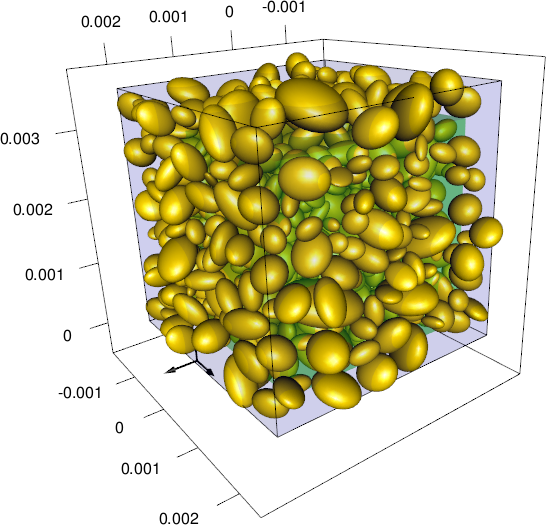
\includegraphics[width=0.5\paperwidth,height=0.5\paperheight,%
keepaspectratio]{periodic_ellipsoids_tighter_fit.png}%
\vfill
}}}

%-------------------------------------------------------
% Versioning
%-------------------------------------------------------
\makeatletter
\def\MyYear#1{%
  \def\yy@##1##2##3##4;{##3##4}%
  \expandafter\yy@#1;
}
\def\MyMonth#1{%
  \def\yy@##1;{0##1}%
  \def\yy@##1##2;{##1##2}%
  \expandafter\yy@#1;
}
\makeatother
\newcommand{\version}{Version \MyYear{\the\year}.\MyMonth{\the\month}}


